%%%%%%%%%%%%%%%%%%%%%%%%%%%%%%%%%%%%%%%%%%%%%%%%%%%%%%%%%%%%%%%%%%%%%%
%% Póster TP final — Finanzas Cuantitativas (FCEN-UBA)
%% Covered Calls y pronósticos de volatilidad: evidencia en SPY y QQQ (2008--2026)
%% Formato: A0 vertical, 3 columnas, una sola hoja. Diseño estilo "Copenhagen".
%% Compilar en Overleaf con pdfLaTeX.
%% Los números salen de numeros.tex y tabla_estrategias.tex (python -m poster.src.build).
%%%%%%%%%%%%%%%%%%%%%%%%%%%%%%%%%%%%%%%%%%%%%%%%%%%%%%%%%%%%%%%%%%%%%%

\documentclass[a0,portrait]{a0poster}
\usepackage[utf8]{inputenc}
\usepackage[T1]{fontenc}
\usepackage[spanish,es-nodecimaldot]{babel}
\usepackage{amsmath, amssymb}

% Tres columnas con línea divisoria
\usepackage{multicol}
\columnsep=45pt
\columnseprule=2pt

% Colores
\usepackage[svgnames]{xcolor}
\definecolor{ku}{RGB}{144,26,30}          % bordó (títulos)
\definecolor{ku-blue}{RGB}{22,69,127}     % azul (subtítulos)
\definecolor{cBH}{HTML}{2A78D6}           % Buy & Hold
\definecolor{cStat}{HTML}{EB6834}         % CC estático
\definecolor{cOTM}{HTML}{8A63D2}          % CC siempre OTM
\definecolor{cMod}{HTML}{1BAF7A}          % CC modelo
\definecolor{ink}{HTML}{0B0B0B}
\definecolor{ink2}{HTML}{52514E}
\def\columnseprulecolor{\color{ku!30}}

\usepackage{times}
\usepackage{graphicx}
\graphicspath{{figures/}}
\usepackage{booktabs, array, multirow}
\usepackage[font=small, labelfont=bf]{caption}
\usepackage{enumitem}
\usepackage{tikz}
\usetikzlibrary{positioning, arrows.meta}

\newcommand{\SPYIV}{20{,}2\%}
\newcommand{\SPYIVcall}{14{,}7\%}
\newcommand{\SPYRV}{16{,}3\%}
\newcommand{\SPYBHCAGR}{11{,}9\%}
\newcommand{\SPYBHSharpe}{0{,}63}
\newcommand{\SPYBHSortino}{0{,}88}
\newcommand{\SPYBHDD}{$-$51\%}
\newcommand{\SPYBHVol}{18{,}5\%}
\newcommand{\SPYBHSold}{0\%}
\newcommand{\SPYBHAporte}{+0{,}0 pp}
\newcommand{\SPYStatCAGR}{5{,}2\%}
\newcommand{\SPYStatSharpe}{0{,}37}
\newcommand{\SPYStatSortino}{0{,}41}
\newcommand{\SPYStatDD}{$-$38\%}
\newcommand{\SPYStatVol}{12{,}2\%}
\newcommand{\SPYStatSold}{100\%}
\newcommand{\SPYStatAporte}{$-$7{,}1 pp}
\newcommand{\SPYOTMCAGR}{9{,}7\%}
\newcommand{\SPYOTMSharpe}{0{,}59}
\newcommand{\SPYOTMSortino}{0{,}74}
\newcommand{\SPYOTMDD}{$-$45\%}
\newcommand{\SPYOTMVol}{15{,}5\%}
\newcommand{\SPYOTMSold}{100\%}
\newcommand{\SPYOTMAporte}{$-$2{,}5 pp}
\newcommand{\SPYModCAGR}{11{,}9\%}
\newcommand{\SPYModSharpe}{0{,}64}
\newcommand{\SPYModSortino}{0{,}88}
\newcommand{\SPYModDD}{$-$51\%}
\newcommand{\SPYModVol}{18{,}3\%}
\newcommand{\SPYModSold}{13\%}
\newcommand{\SPYModAporte}{+0{,}0 pp}
\newcommand{\SPYVsBH}{+0{,}0 pp}
\newcommand{\SPYVsBHCI}{[$-$0{,}8; +0{,}7]}
\newcommand{\SPYVsOTM}{+2{,}5 pp}
\newcommand{\SPYVsOTMCI}{[+0{,}2; +5{,}0]}
\newcommand{\SPYVsStat}{+7{,}2 pp}
\newcommand{\SPYVsStatCI}{[+3{,}4; +11{,}0]}
\newcommand{\SPYPSRactivo}{0{,}50}
\newcommand{\SPYDSR}{0{,}96}
\newcommand{\SPYQlikeKalman}{0{,}43}
\newcommand{\SPYQlikeIV}{0{,}44}
\newcommand{\SPYQlikeEns}{0{,}47}
\newcommand{\QQQIV}{22{,}8\%}
\newcommand{\QQQIVcall}{16{,}7\%}
\newcommand{\QQQRV}{19{,}7\%}
\newcommand{\QQQBHCAGR}{16{,}9\%}
\newcommand{\QQQBHSharpe}{0{,}78}
\newcommand{\QQQBHSortino}{1{,}17}
\newcommand{\QQQBHDD}{$-$49\%}
\newcommand{\QQQBHVol}{21{,}2\%}
\newcommand{\QQQBHSold}{0\%}
\newcommand{\QQQBHAporte}{+0{,}0 pp}
\newcommand{\QQQStatCAGR}{5{,}3\%}
\newcommand{\QQQStatSharpe}{0{,}36}
\newcommand{\QQQStatSortino}{0{,}42}
\newcommand{\QQQStatDD}{$-$41\%}
\newcommand{\QQQStatVol}{12{,}8\%}
\newcommand{\QQQStatSold}{100\%}
\newcommand{\QQQStatAporte}{$-$12{,}0 pp}
\newcommand{\QQQOTMCAGR}{10{,}5\%}
\newcommand{\QQQOTMSharpe}{0{,}60}
\newcommand{\QQQOTMSortino}{0{,}78}
\newcommand{\QQQOTMDD}{$-$47\%}
\newcommand{\QQQOTMVol}{16{,}7\%}
\newcommand{\QQQOTMSold}{100\%}
\newcommand{\QQQOTMAporte}{$-$6{,}5 pp}
\newcommand{\QQQModCAGR}{16{,}9\%}
\newcommand{\QQQModSharpe}{0{,}79}
\newcommand{\QQQModSortino}{1{,}17}
\newcommand{\QQQModDD}{$-$49\%}
\newcommand{\QQQModVol}{21{,}0\%}
\newcommand{\QQQModSold}{9\%}
\newcommand{\QQQModAporte}{$-$0{,}1 pp}
\newcommand{\QQQVsBH}{$-$0{,}1 pp}
\newcommand{\QQQVsBHCI}{[$-$1{,}1; +0{,}8]}
\newcommand{\QQQVsOTM}{+6{,}5 pp}
\newcommand{\QQQVsOTMCI}{[+3{,}6; +9{,}6]}
\newcommand{\QQQVsStat}{+11{,}9 pp}
\newcommand{\QQQVsStatCI}{[+7{,}3; +16{,}8]}
\newcommand{\QQQPSRactivo}{0{,}45}
\newcommand{\QQQDSR}{0{,}99}
\newcommand{\QQQQlikeKalman}{0{,}32}
\newcommand{\QQQQlikeIV}{0{,}31}
\newcommand{\QQQQlikeEns}{0{,}35}
\newcommand{\NCycles}{224}
\newcommand{\NTrials}{36}
\newcommand{\SkewA}{0{,}83}
\newcommand{\SkewB}{0{,}18}
\newcommand{\SkewN}{821}
\newcommand{\PBPcorr}{0{,}97}
\newcommand{\PBPsim}{6{,}3\%}
\newcommand{\PBPbruto}{6{,}6\%}
\newcommand{\EarlyCost}{1{,}1 pp}
\newcommand{\VrpGK}{6{,}6 pp}
\newcommand{\VrpYZ}{3{,}2 pp}
\newcommand{\OUhalflife}{7}
\newcommand{\OUstress}{3{,}4\%}
\newcommand{\DoptSPY}{0{,}50}
\newcommand{\DoptQQQ}{0{,}50}
\newcommand{\DoptNVDA}{0{,}10}


\newcommand{\iq}{\textquestiondown}

% Títulos de sección: sin cortes con guion y alineados a la izquierda
\makeatletter
\renewcommand{\section}[1]{%
  \par\vfill\vspace{0.8cm}%  % \vfill: reparte el espacio libre entre secciones (columnas parejas)
  {\noindent\raggedright\hyphenpenalty=10000\exhyphenpenalty=10000\color{ku}\Large\bfseries #1\par}%
  \vspace{0.35cm}\noindent}
\renewcommand{\subsection}[1]{%
  \par\vspace{0.5cm}%
  {\noindent\raggedright\hyphenpenalty=10000\color{ku-blue}\large\bfseries #1\par}%
  \vspace{0.2cm}\noindent}
\makeatother

% Recuadro destacado
\newcommand{\destacado}[1]{%
  \begin{center}\fcolorbox{ku}{white!95!ku}{\parbox{0.94\linewidth}{\centering #1}}\end{center}}

\setlength{\parindent}{0pt}
\setlength{\parskip}{0.4em}
\setlist{leftmargin=*, itemsep=0.25em, topsep=0.3em}

\begin{document}

%----------------------------------------------------------------------------------------
%	ENCABEZADO
%----------------------------------------------------------------------------------------
\begin{minipage}[t]{0.72\linewidth}
  \vspace{0pt}
  {\VeryHuge\color{ku}\bfseries Covered Calls y pronósticos\\[0.2cm] de volatilidad}\\[0.6cm]
  {\huge\bfseries Evidencia en SPY y QQQ (2008--2026)}\\[0.7cm]
  {\LARGE\bfseries Renato Trucillo Biglieri \quad [Autores del grupo]}\\[0.3cm]
  {\Large Finanzas Cuantitativas --- Prof.\ Guido Schifani $\cdot$ FCEN, Universidad de Buenos Aires}
\end{minipage}%
\begin{minipage}[t]{0.28\linewidth}
  \vspace{0pt}
  \raggedleft\color{DarkSlateGray}
  {\LARGE\bfseries Universidad de Buenos Aires}\\[0.25cm]
  {\Large Facultad de Ciencias Exactas\\ y Naturales}\\[0.25cm]
  {\Large Departamento de Matemática / Computación}\\[0.3cm]
  {\large\ttfamily renatrucillo8@gmail.com}
\end{minipage}

\vspace{0.8cm}
{\color{ku}\rule{\linewidth}{5pt}}
\vspace{0.2cm}

%----------------------------------------------------------------------------------------
%	CUERPO EN TRES COLUMNAS
%----------------------------------------------------------------------------------------
\begin{multicols*}{3}

% =====================================================================  COLUMNA 1
\section{Introducción}

Una \textbf{Covered Call} consiste en comprar un activo y, al mismo tiempo, \textbf{vender una opción call}: se le da a otro el derecho a comprarnos el activo a un precio fijo $K$ (\textit{strike}). A cambio, se \textbf{cobra una prima por adelantado}.

Si el activo cae o se estanca, la prima amortigua la pérdida; si sube con fuerza, la ganancia queda cortada en $K$. Es una de las estrategias con opciones más populares, promocionada como una forma de ``cobrar una renta'' todos los meses.

La pregunta de fondo es directa:
\begin{itemize}
  \item \textbf{\iq{}Esa prima compensa, a largo plazo, las subas que se resignan?}
  \item Y si no siempre lo hace, \textbf{\iq{}puede un pronóstico de volatilidad decirnos cuándo conviene vender la call y cuándo no?}
\end{itemize}

\begin{center}
  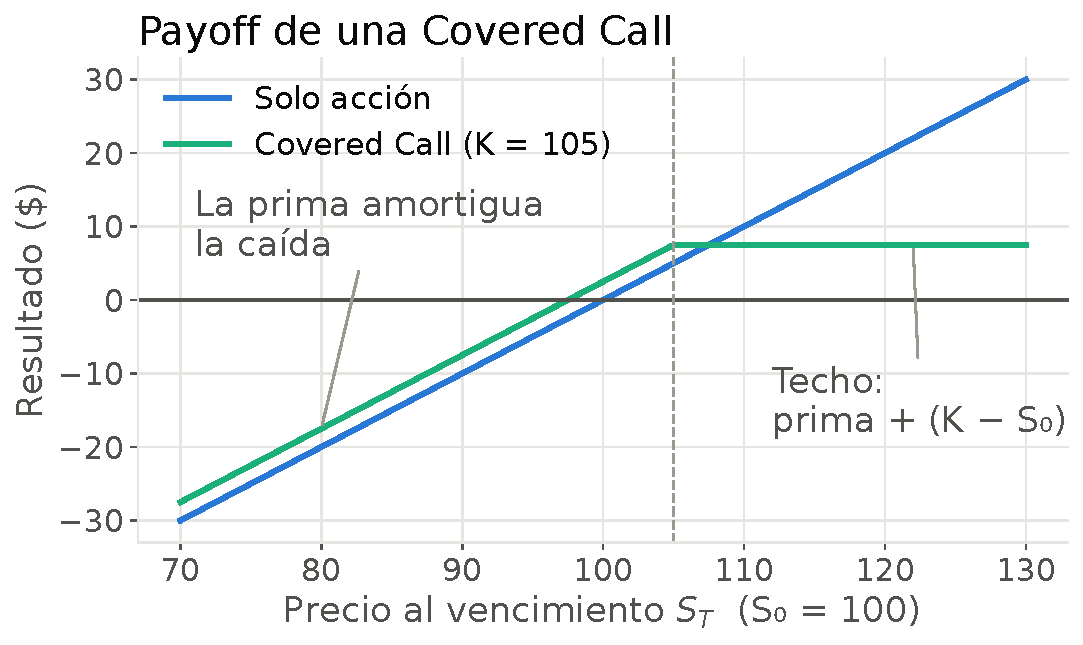
\includegraphics[width=0.95\linewidth]{01_payoff.pdf}
  \captionof{figure}{\textbf{Payoff al vencimiento:} $\protect\min(S_T,\,K)-S_0+C_0$. La prima atenúa las pérdidas leves pero corta la ganancia en el strike $K$.}
\end{center}

\section{Pregunta e hipótesis}

El valor de la prima depende de la \textbf{volatilidad implícita} (IV). Si después el activo se mueve menos de lo que la prima descontaba, el vendedor de la call gana.

\destacado{\textbf{Hipótesis:} vender la call \textbf{solo si} nuestro pronóstico $\hat\sigma$ es \textbf{menor} que la volatilidad implícita \textbf{de esa call}, $\text{IV}(K)$.}

\begin{enumerate}
  \item Pronosticar la volatilidad sin mirar el futuro (\textit{walk-forward}).
  \item Medir a qué volatilidad se venden realmente las calls (\textit{skew}).
  \item Comparar contra \textbf{Buy \& Hold}, \textbf{CC estático ATM} y \textbf{CC siempre OTM} (regla sin modelo).
  \item Controlar el sobreajuste con el \textit{Deflated Sharpe Ratio}.
\end{enumerate}

\section{Datos}

\textbf{SPY} (S\&P~500, IV $=$ VIX) y \textbf{QQQ} (Nasdaq-100, IV $=$ VXN).
\begin{itemize}
  \item \textbf{\NCycles{} ciclos mensuales} fuera de muestra (ene-2008 a sep-2026, con 2007 de calentamiento): se vende al cierre del vencimiento estándar (tercer viernes) y se liquida en el siguiente. Incluye 2008, el Covid y 2022.
  \item \textbf{Fuentes:} Excel de la cátedra (SPY, VIX); Yahoo Finance (QQQ, VXN, T-bill \^{}IRX, ETF PBP); Interactive Brokers (\SkewN{} calls de SPX para calibrar el \textit{skew}).
\end{itemize}

\section{Metodología}

\begin{center}
\begin{tikzpicture}[node distance=5mm, every node/.style={font=\normalsize},
   box/.style={draw=ku, fill=white!95!ku, rounded corners=3mm, thick, align=center, text width=0.86\columnwidth, minimum height=13mm, inner sep=2mm},
   hl/.style={box, draw=cMod, fill=cMod!12},
   arr/.style={-{Latex[length=4mm]}, very thick, color=ink2}]
  \node[box] (a) {Retornos OHLC diarios hasta \mbox{$t_0-1$}};
  \node[box, below=of a] (b) {5 modelos de volatilidad \mbox{$\longrightarrow$} \textbf{ensamble} \mbox{$\hat\sigma$}};
  \node[hl, below=of b] (c) {IV de la call: \mbox{$\text{IV}(K)=\text{VIX}\cdot(\SkewA-\SkewB\,x)$}};
  \node[hl, below=of c] (d) {\mbox{\iq{}$\hat\sigma<\text{IV}(K)$?\ $\Longrightarrow$\ \textbf{vender la call}}};
  \node[hl, below=of d] (e) {Strike \mbox{$K=S_0\,e^{\,0{,}5\,\hat\sigma\sqrt{T}}$}};
  \node[box, below=of e] (f) {Black-Scholes $+$ ejercicio anticipado\\ antes del dividendo};
  \node[box, below=of f] (g) {P\&L del ciclo y drawdown diario};
  \foreach \i/\j in {a/b,b/c,c/d,d/e,e/f,f/g} \draw[arr] (\i) -- (\j);
\end{tikzpicture}
\captionof{figure}{\textbf{Flujo de decisión del modelo en cada ciclo.}}
\end{center}

$x=\ln(K/S)/(\text{VIX}\sqrt{T})$ es la distancia al strike en desvíos. Todo es \textbf{walk-forward} (ventana expansiva); volatilidades realizadas en base 252 ruedas e IV en base 365 días. Costo: 2\% de la prima.

\textbf{Validación:} el CC estático simulado replica al ETF real PBP (BuyWrite) con correlación \PBPcorr{} y rendimiento anual \PBPsim{} vs.\ \PBPbruto{} antes de comisiones.

\columnbreak

% =====================================================================  COLUMNA 2
\section{\iq{}A qué IV se vende la call? El skew}

\begin{center}
  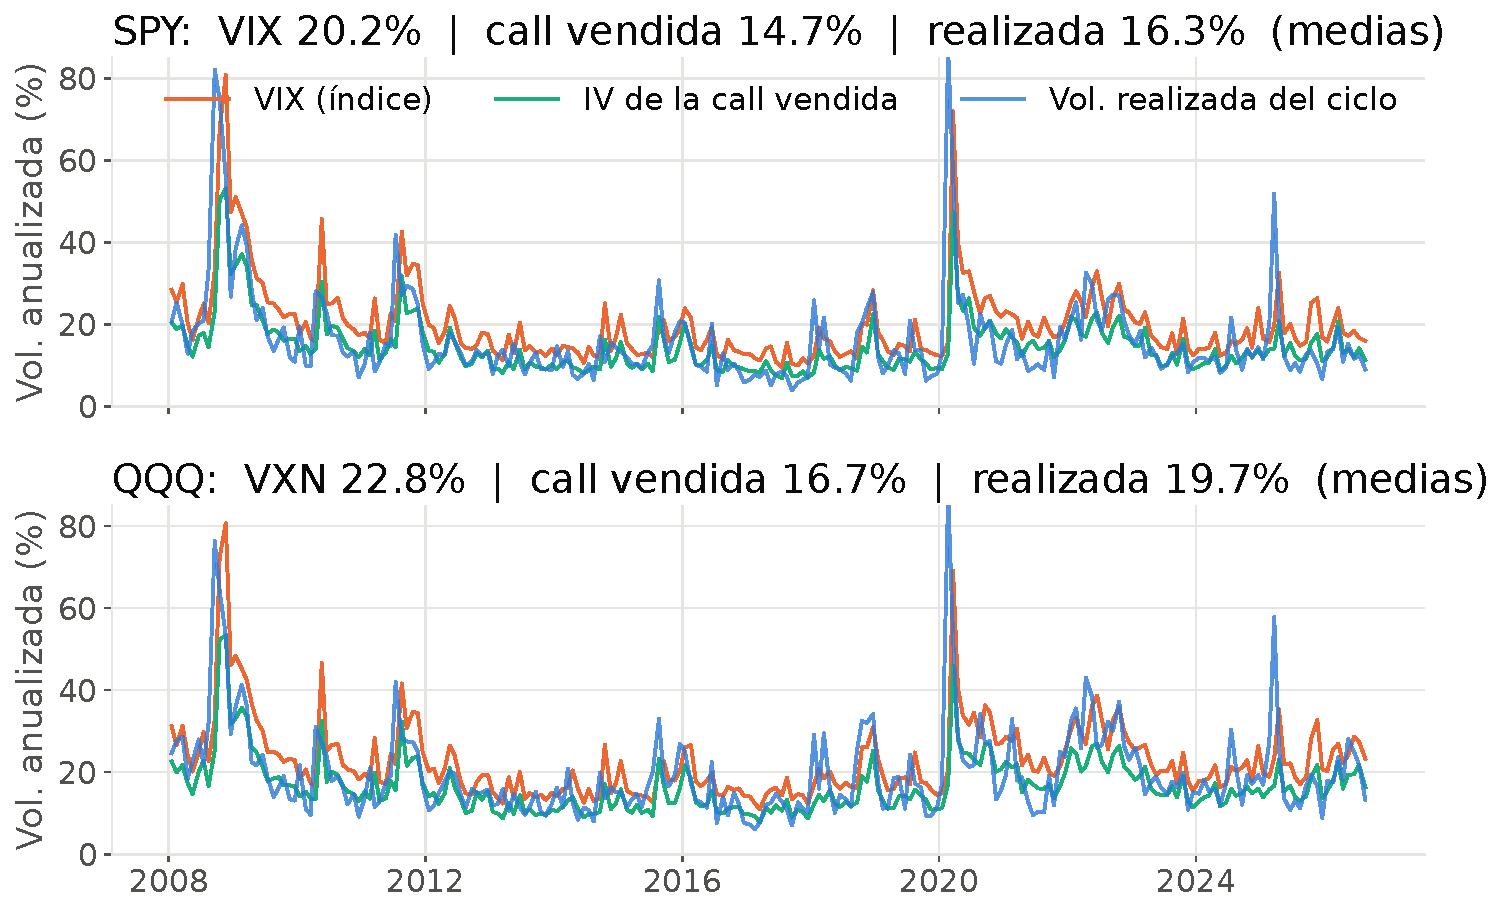
\includegraphics[width=\linewidth]{03_iv_call_vs_realizada.pdf}
  \captionof{figure}{\textbf{VIX, IV de la call y volatilidad realizada:} el VIX (naranja) supera a la realizada (azul), pero la call que se vende (verde) cotiza por debajo de ambas.}
\end{center}

En SPY el VIX promedia \SPYIV{} y la volatilidad realizada \SPYRV: parece haber margen. Pero la \textbf{call vendida cotiza en promedio a \SPYIVcall} (QQQ: \QQQIVcall{} vs.\ \QQQRV{} realizada). El VIX está ``inflado'' por los \textbf{puts}, caros porque protegen de las caídas (\textit{skew}).

\destacado{\color{ku}\bfseries La prima de volatilidad está en los puts, no en las calls.}

\section{Calidad de los pronósticos}

\begin{center}
  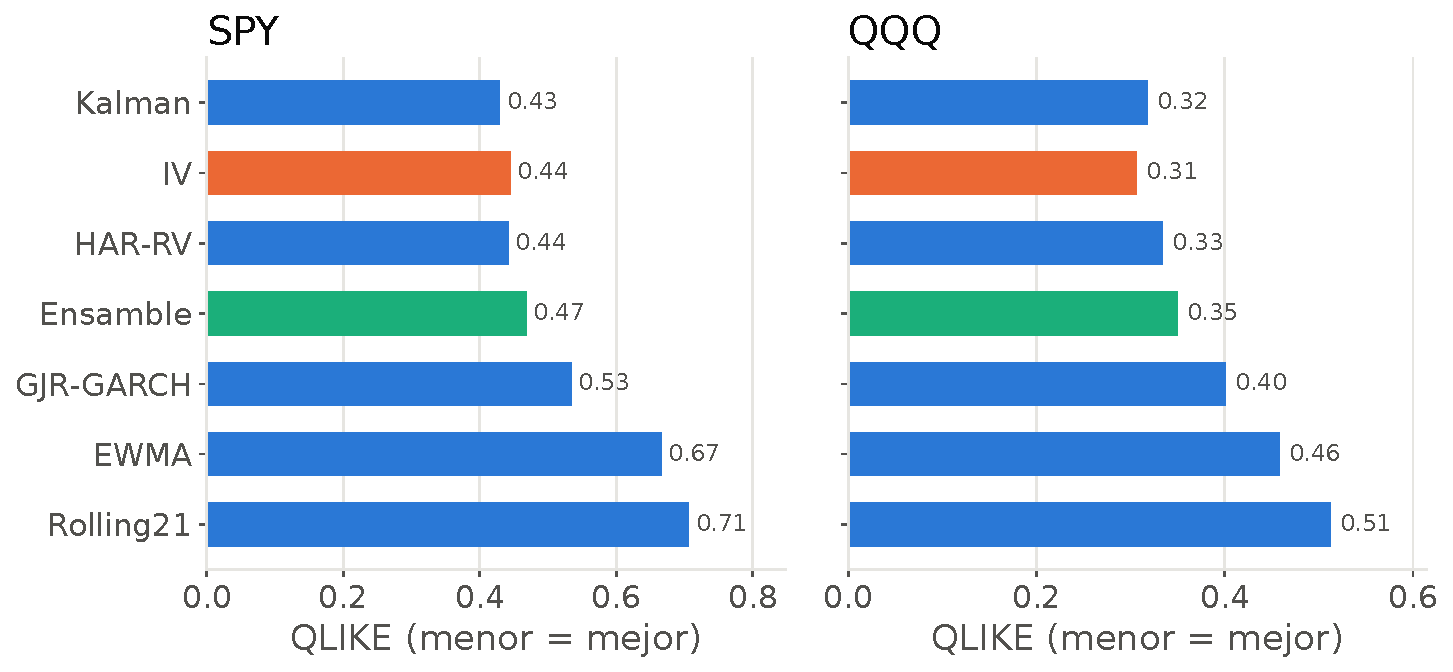
\includegraphics[width=\linewidth]{04_error_pronostico.pdf}
  \captionof{figure}{\textbf{Error QLIKE fuera de muestra (menor es mejor):} el Kalman (SPY: \SPYQlikeKalman) empata con la IV (\SPYQlikeIV); el ensamble (\SPYQlikeEns) queda cerca de los mejores.}
\end{center}

\subsection{Los 5 modelos de volatilidad}
{\small
\renewcommand{\arraystretch}{1.2}
\begin{tabular}{@{}p{0.25\linewidth}p{0.71\linewidth}@{}}
  \toprule
  \textbf{Modelo} & \textbf{Idea} \\ \midrule
  Rolling 21d & desvío de los últimos 21 retornos \\
  EWMA & $\sigma^2_t=\lambda\sigma^2_{t-1}+(1-\lambda)r^2_{t-1}$, $\lambda=0{,}97$ \\
  GJR-GARCH & $\sigma^2_t=\omega+(\alpha+\gamma\mathbf 1_{r<0})r^2_{t-1}+\beta\sigma^2_{t-1}$ \\
  HAR-RV & regresión sobre volatilidad diaria, semanal y mensual \\
  Kalman & log-varianza latente AR(1), estimada por MV \\
  Ensamble & promedio de las varianzas de los 5 modelos \\ \bottomrule
\end{tabular}\par}

\section{Fase 1: features de volatilidad}

\begin{center}
  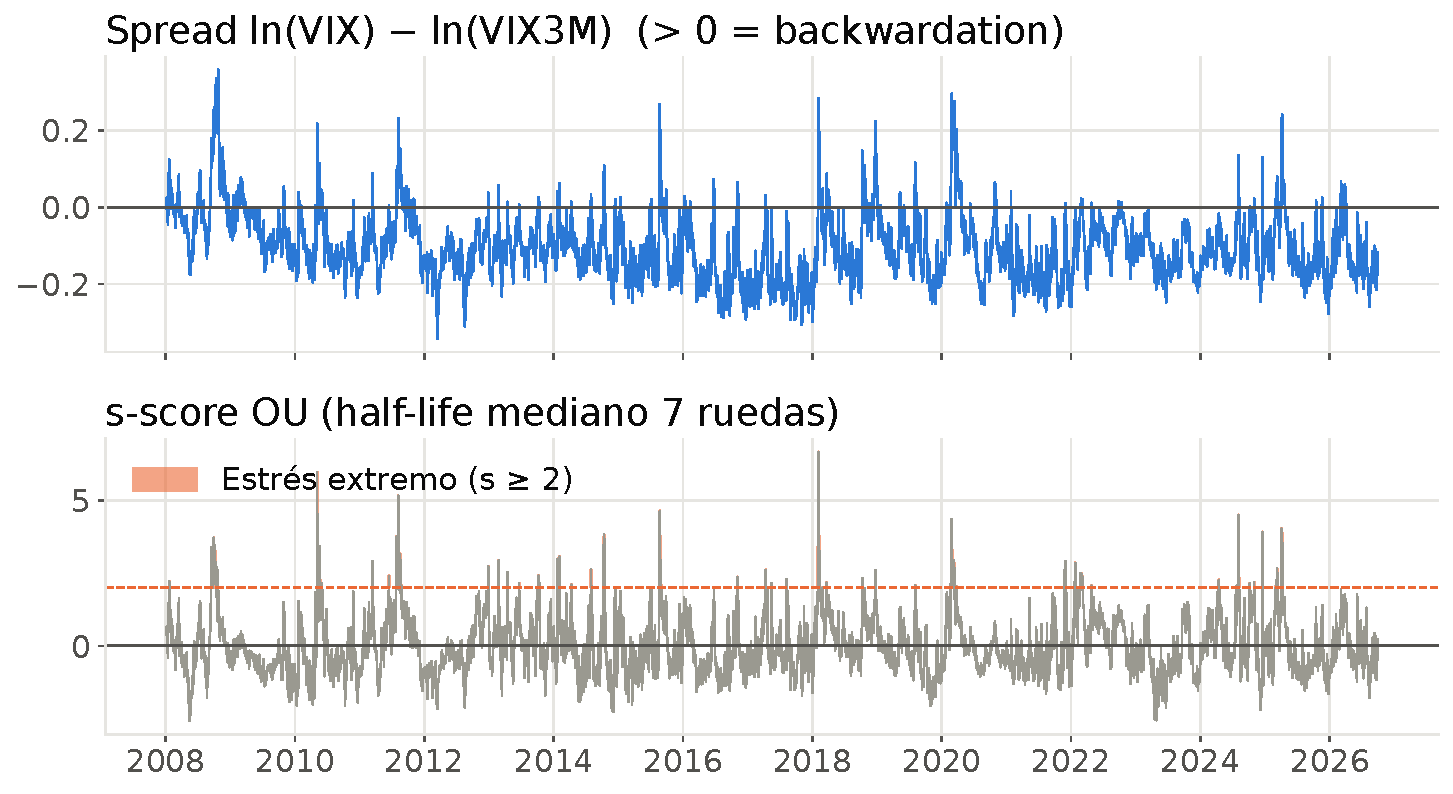
\includegraphics[width=\linewidth]{fase1_ou_sscore.pdf}
  \captionof{figure}{\textbf{Estructura temporal del VIX:} spread $\ln\text{VIX}-\ln\text{VIX3M}$ y su s-score de Ornstein-Uhlenbeck.}
\end{center}

\begin{itemize}
  \item \textbf{Ornstein-Uhlenbeck:} half-life de $\approx$\,\OUhalflife{} ruedas (con corrección de sesgo); estrés extremo ($s\ge2$) solo el \OUstress{} de los días.
  \item \textbf{Prima de varianza ex-ante:} VIX $-$ Yang-Zhang $=$ \VrpYZ. Con Garman-Klass daría \VrpGK, porque ignora el salto entre el cierre y la apertura.
  \item \textbf{Diferenciación fraccionaria} (log-precio, $d^*$ elegido con 2007--2014): $d^*=$ \DoptSPY{} en SPY y QQQ, \DoptNVDA{} en NVDA.
\end{itemize}

\columnbreak

% =====================================================================  COLUMNA 3
\section{Resultado: crecimiento de \$1}

\begin{center}
  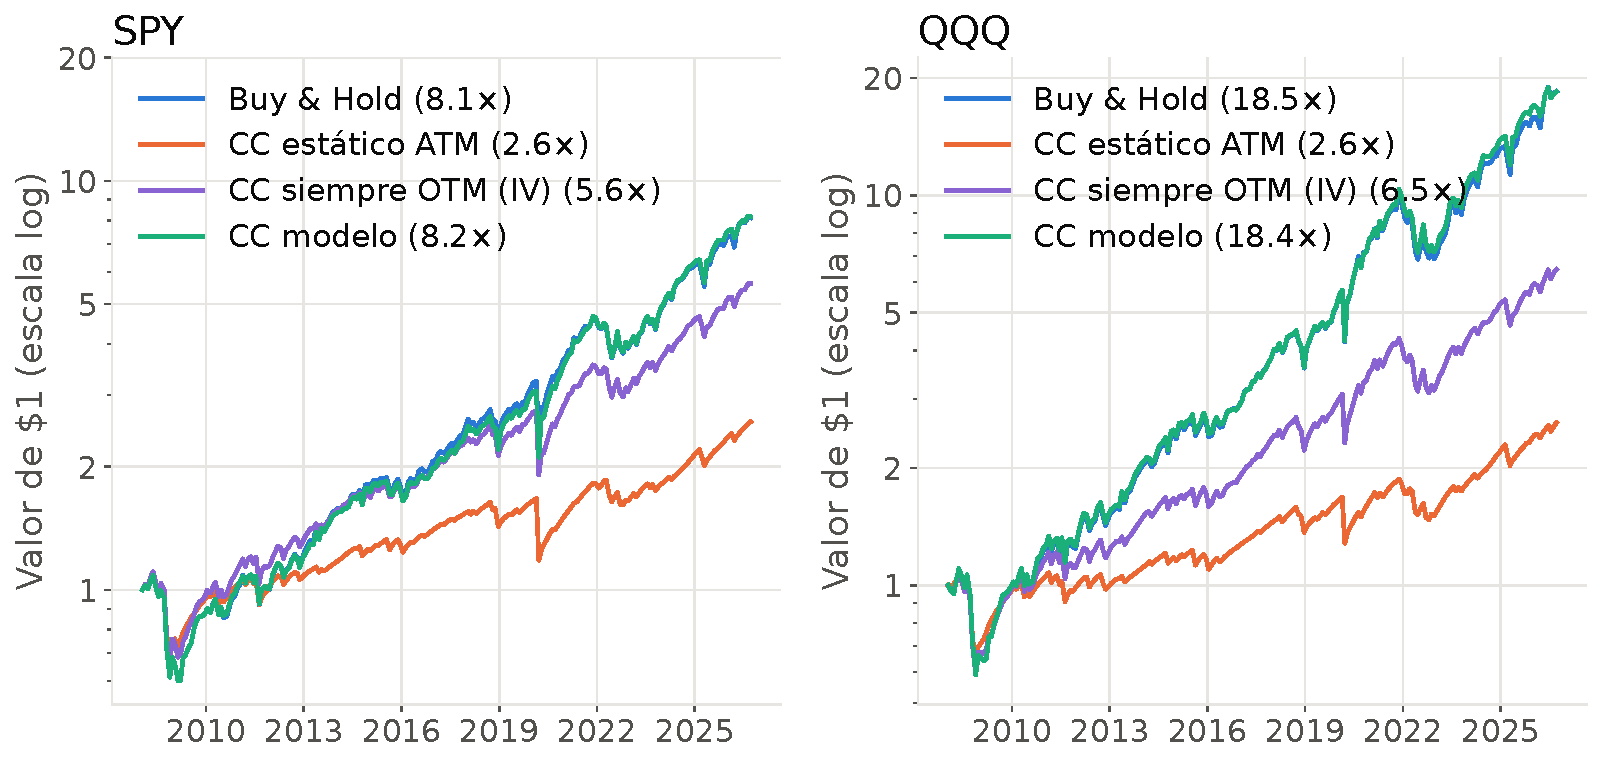
\includegraphics[width=\linewidth]{06_crecimiento.pdf}
  \captionof{figure}{\textbf{Crecimiento de \$1 (2008--2026):} escala logarítmica, retorno total. El CC modelo se superpone con el Buy \& Hold; vender siempre queda claramente abajo.}
\end{center}

\section{Estrategias comparadas}

\begin{center}
{\small
\renewcommand{\arraystretch}{1.2}
\setlength{\tabcolsep}{5pt}
\begin{tabular}{@{}llrrrrrr@{}}
\toprule
& & \textbf{CAGR} & \textbf{Vol.} & \textbf{Sharpe} & \textbf{Sortino} & \textbf{MaxDD} & \textbf{Vende} \\ \midrule
\multirow{4}{*}{\textbf{SPY}} & Buy \& Hold & 11{,}9\% & 18{,}5\% & 0{,}63 & 0{,}88 & $-$51\% & -- \\
 & CC estático ATM & 5{,}2\% & 12{,}2\% & 0{,}37 & 0{,}41 & $-$38\% & 100\% \\
 & CC siempre OTM & 9{,}7\% & 15{,}5\% & 0{,}59 & 0{,}74 & $-$45\% & 100\% \\
 & \textbf{CC modelo} & 11{,}9\% & 18{,}3\% & 0{,}64 & 0{,}88 & $-$51\% & 13\% \\
\midrule
\multirow{4}{*}{\textbf{QQQ}} & Buy \& Hold & 16{,}9\% & 21{,}2\% & 0{,}78 & 1{,}17 & $-$49\% & -- \\
 & CC estático ATM & 5{,}3\% & 12{,}8\% & 0{,}36 & 0{,}42 & $-$41\% & 100\% \\
 & CC siempre OTM & 10{,}5\% & 16{,}7\% & 0{,}60 & 0{,}78 & $-$47\% & 100\% \\
 & \textbf{CC modelo} & 16{,}9\% & 21{,}0\% & 0{,}79 & 1{,}17 & $-$49\% & 9\% \\
\bottomrule
\end{tabular}
\par}
\captionof{table}{\textbf{Desempeño fuera de muestra (\NCycles{} ciclos).} MaxDD diario, con la call valuada a mercado; Sharpe y Sortino sobre excesos. CC siempre OTM: vende todos los meses con el mismo tipo de strike, usando la IV en lugar del modelo.}
\end{center}

\section{\iq{}Qué aporta el modelo?}

\begin{center}
{\small
\renewcommand{\arraystretch}{1.2}
\begin{tabular}{@{}lcc@{}}
  \toprule
  \textbf{CC modelo menos\ldots} (pp/año) & \textbf{SPY} & \textbf{QQQ} \\ \midrule
  Buy \& Hold & \SPYVsBH{} {\footnotesize\SPYVsBHCI} & \QQQVsBH{} {\footnotesize\QQQVsBHCI} \\
  CC siempre OTM & \SPYVsOTM{} {\footnotesize\SPYVsOTMCI} & \QQQVsOTM{} {\footnotesize\QQQVsOTMCI} \\
  CC estático ATM & \SPYVsStat{} {\footnotesize\SPYVsStatCI} & \QQQVsStat{} {\footnotesize\QQQVsStatCI} \\ \bottomrule
\end{tabular}\par}
\captionof{table}{\textbf{Diferencia anual de retorno} con IC 95\% (bootstrap estacionario, bloques de 3 meses).}
\end{center}

El modelo vende solo el \textbf{\SPYModSold} de los meses en SPY (\QQQModSold{} en QQQ). Le gana a vender siempre, pero \textbf{no se distingue del Buy \& Hold}: la probabilidad de superarlo es \SPYPSRactivo{} en SPY y \QQQPSRactivo{} en QQQ, tras probar \NTrials{} configuraciones.

\section{Conclusiones}

\begin{itemize}[itemsep=0.5em]
  \item \textbf{Vender calls todos los meses rindió menos que quedarse con el índice:} la call ATM restó \SPYStatAporte{} por año en SPY y \QQQStatAporte{} en QQQ.
  \item \textbf{\iq{}Por qué?} La ``prima de volatilidad'' del VIX es el precio del seguro contra caídas (los puts). Las calls se venden baratas: a \SPYIVcall, cuando el mercado después se movió \SPYRV.
  \item \textbf{Un buen pronóstico sirve, pero para saber cuándo no vender:} bien planteado, el modelo casi nunca vende y termina igual que el Buy \& Hold.
  \item \textbf{En la práctica:} en índices, la Covered Call no se justifica por la prima; si se usa, que sea sabiendo que cuesta rendimiento.
\end{itemize}

{\small\textbf{Limitaciones:} skew calibrado con un solo período (jun--sep 2026) y aplicado también a QQQ; precios teóricos con costo fijo; solo dos índices. El ejercicio anticipado antes del dividendo le cuesta \EarlyCost{} por año al CC estático en SPY.\par}

\section{Referencias}
{\footnotesize
Hull (2018), \textit{Options, Futures and Other Derivatives}. \;
Glosten, Jagannathan \& Runkle (1993), \textit{J.\ Finance}. \;
J.P.\ Morgan/Reuters (1996), \textit{RiskMetrics}. \;
Corsi (2009), \textit{J.\ Financial Econometrics}. \;
Garman \& Klass (1980), \textit{J.\ Business}. \;
Yang \& Zhang (2000), \textit{J.\ Business}. \;
Bollerslev, Tauchen \& Zhou (2009), \textit{Rev.\ Financial Studies}. \;
Whaley (2002), \textit{J.\ Derivatives}. \;
Israelov \& Nielsen (2015), \textit{Financial Analysts J.} \;
Politis \& Romano (1994), \textit{JASA}. \;
Bailey \& López de Prado (2014), \textit{J.\ Portfolio Management}. \;
López de Prado (2018), \textit{Advances in Financial Machine Learning}.\par}

\end{multicols*}

\end{document}
